\documentclass[tikz,border=5pt]{standalone}
\usepackage[UTF8]{ctex}
\usepackage{amsmath,amssymb}
\usetikzlibrary{arrows.meta,calc,angles,quotes,patterns,decorations.pathmorphing}
\definecolor{field}{HTML}{176B9B}
\definecolor{force}{HTML}{B64B32}
\tikzset{>=Latex,line width=.8pt,every node/.style={font=\small},field/.style={color=field},force/.style={color=force},body/.style={draw=black,fill=blue!6},ghost/.style={dashed,gray},labelbox/.style={fill=white,inner sep=1.5pt}}
\begin{document}
\begin{tikzpicture}
% Hollow thin wall: front annulus and inner opening, not solid end caps.
\draw[ghost](-2,0)ellipse(.4 and 1.25);
\draw[ghost](-2,0)ellipse(.36 and 1.12);
\fill[blue!5](-2,1.12)rectangle(2,1.25);
\fill[blue!5](-2,-1.25)rectangle(2,-1.12);
\draw(-2,1.25)--(2,1.25);\draw(-2,-1.25)--(2,-1.25);
\draw[ghost](-2,1.12)--(2,1.12);\draw[ghost](-2,-1.12)--(2,-1.12);
\path[fill=blue!15,even odd rule](2,0)ellipse(.4 and 1.25)(2,0)ellipse(.36 and 1.12);
\draw(2,0)ellipse(.4 and 1.25);\draw(2,0)ellipse(.36 and 1.12);
\draw[->,field,thick](-1.6,0)--(2.9,0)node[right]{$B,+z$};
\draw[force,->](2,1.05)arc(90:300:.33 and 1.05);
\node[right]at(2.6,.8){$I$};
\draw[<->](-2,-1.7)--(2,-1.7)node[midway,below]{$l$};
\draw[<->](2,0)--(2,1.12)node[midway,left=1pt]{$r$};
\node[above]at(0,1.6){薄壁 $d\ll r$};
\end{tikzpicture}
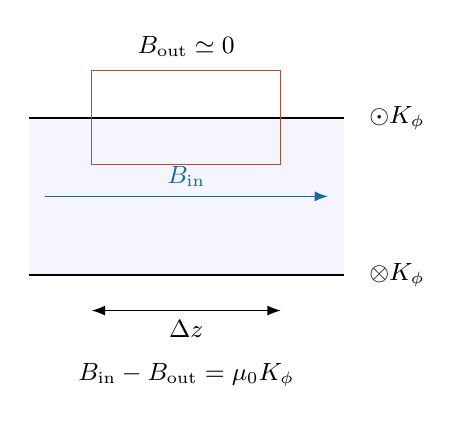
\begin{tikzpicture}
\fill[blue!4](-2,-1)rectangle(2,1);
\draw[thick](-2,-1)--(2,-1);\draw[thick](-2,1)--(2,1);
\draw[->,field](-1.8,0)--(1.8,0)node[midway,above]{$B_{\rm in}$};
\draw[force,->](-1.2,.4)--(1.2,.4)--(1.2,1.6)--(-1.2,1.6)--cycle;
\node[above]at(0,1.65){$B_{\rm out}\simeq0$};
\draw[<->](-1.2,-1.45)--(1.2,-1.45)node[midway,below]{$\Delta z$};
\node[right]at(2.2,1){$\odot K_\phi$};
\node[right]at(2.2,-1){$\otimes K_\phi$};
\node[below]at(0,-2){$B_{\rm in}-B_{\rm out}=\mu_0K_\phi$};
\end{tikzpicture}
\begin{tikzpicture}
\draw[body](0,0)circle(1.4);
\foreach\a in{0,60,120,180,240,300}
\node[field]at({.65*cos(\a)},{.65*sin(\a)}){$\odot$};
\node[field]at(2.4,1.4){$B_z>0,\;\dot B_z<0$};
\draw[force,->,thick](1.7,0)arc(0:80:1.7);
\draw[force,->,thick](-1.7,0)arc(180:260:1.7);
\node[force,left]at(-1.7,.9){$E_\phi>0$};
\draw[->](0,0)--(1.4,0)node[midway,below]{$r$};
\node[below]at(0,-2.15){从 $+z$ 端观察，正环流逆时针};
\end{tikzpicture}
\begin{tikzpicture}
\draw[->](0,0)--(6,0)node[right]{$t/\tau_c$};
\draw[->](0,0)--(0,3)node[above]{归一化量};
\draw[field,thick,domain=0:5.5,samples=80]plot(\x,{2.6*exp(-\x)});
\draw[force,thick,domain=0:5.5,samples=80]plot(\x,{2.6*exp(-2*\x)});
\draw[green!50!black,thick,domain=0:5.5,samples=80]plot(\x,{2.6*(1-exp(-2*\x))});
\node[field,right]at(1.5,1.1){$I/I_0$};
\node[force,right]at(2,.6){$W_B/W_B(0)$};
\node[green!50!black,right]at(2,2.8){$Q/W_B(0)$};
\node[left]at(0,2.6){$1$};
\end{tikzpicture}
\end{document}
